\documentclass{beamer}
\usepackage{xcolor}
\usepackage[utf8]{inputenc}
\usepackage[english]{babel} 
\usepackage{listings}

\usepackage{parcolumns}


\usetheme{Madrid}
\usecolortheme{beaver}

\beamertemplatenavigationsymbolsempty

\renewcommand{\emph}{\textcolor{red}}

%------------------------------------------------------------
%This block of code defines the information to appear in the
%Title page
\title[Resource Sharing] %optional
{Enabling resource sharing in dataflow circuits}

\author[Marmet] % (optional)
{Axel Marmet}

\institute[EPFL] % (optional)

\date[EPFL 2019] % (optional)

%\logo{
\includegraphics[height=1cm]{EPFL_Logo_Digital_RGB_PROD-768x333.png}}

%End of title page configuration block
%------------------------------------------------------------



%------------------------------------------------------------
%The next block of commands puts the table of contents at the 
%beginning of each section and highlights the current section:

%\AtBeginSection[]
%{
%  \begin{frame}
%    \frametitle{Table of Contents}
%    \tableofcontents[currentsection]
%  \end{frame}
%}
%------------------------------------------------------------


\begin{document}

%The next statement creates the title page.
\frame{\titlepage}


%---------------------------------------------------------
%This block of code is for the table of contents after
%the title page
%\begin{frame}
%\frametitle{Table of Contents}
%\tableofcontents
%\end{frame}
%---------------------------------------------------------

\section{Basic Idea}
\begin{frame}[fragile]
\frametitle{Motivation}
\begin{columns}[T]
    \begin{column}{0.45\textwidth}
      \begin{itemize}
          \item New iteration every two clock cycles
          \item Each multiplier has an occupancy of $0.5$
          \item Using only one multiplier would not hurt performance but diminish size of circuit
      \end{itemize}
    \end{column}
    \begin{column}{0.1\textwidth}
    \end{column}
    \begin{column}{0.45\textwidth}
      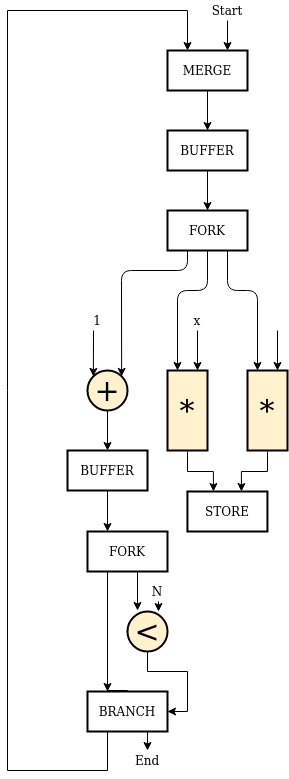
\includegraphics[scale=0.28]{base_case.png}
    \end{column}
  \end{columns}
\end{frame}

\begin{frame}[fragile]
\frametitle{Initial idea}
\begin{columns}[T]
    \begin{column}{0.45\textwidth}
    We add two new components to enable sharing \newline
    \begin{description}
        \item[Selector] Responsible for selecting inputs in a way that ensures fairness and will never deadlock
        \item[Distributor] Must send the resulting token to the correct outputs, is told where to send by the Selector through a FIFO
    \end{description}
    \end{column}
    \begin{column}{0.1\textwidth}
    \end{column}
    \begin{column}{0.45\textwidth}
      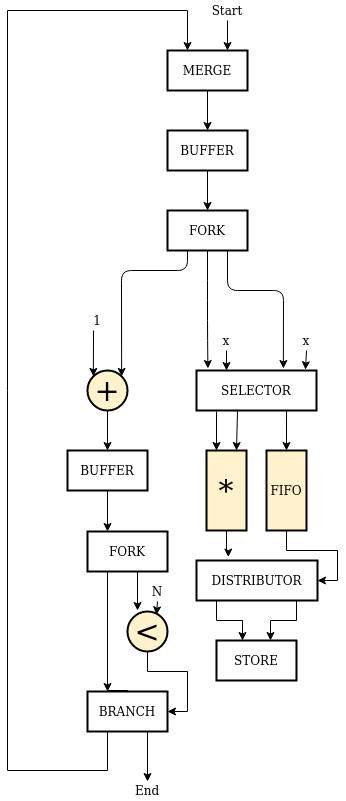
\includegraphics[scale=0.28]{shared_base_case.png}
    \end{column}
  \end{columns}
\end{frame}

\begin{frame}{Deadlock avoidance}
  How to schedule execution without causing deadlock ?
  \begin{columns}[T]
    \begin{column}{0.25\textwidth}
      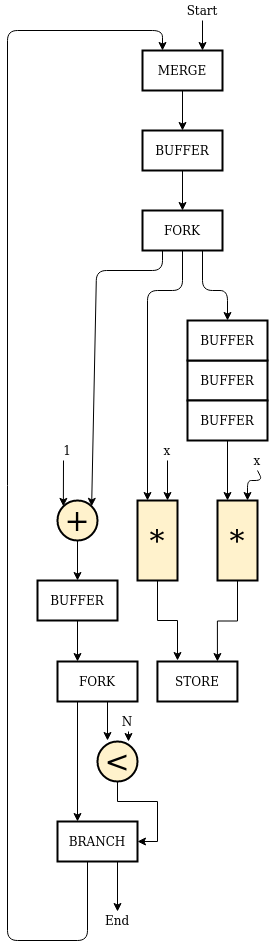
\includegraphics[scale=0.25]{blocking_unshared.png}
    \end{column}
    \begin{column}{0.1\textwidth}
    \begin{center}
        becomes
    \end{center}
    \end{column}
    \begin{column}{0.25\textwidth}
      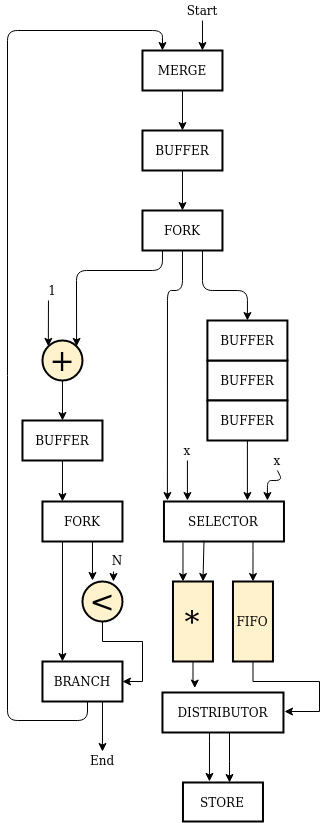
\includegraphics[scale=0.25]{blocking_shared.png}
    \end{column}
  \end{columns}
\end{frame}

\begin{frame}{Enforcing all transactions firing}
\begin{columns}
    \begin{column}{0.45\textwidth}
    We must enforce that all transactions from one BB happen before any from another BB (or the same in another iteration) \newline \newline
    We use the same mechanism as LSQs to be informed of ...
    \end{column}
    \begin{column}{0.1\textwidth}
    \end{column}
    \begin{column}{0.45\textwidth}
      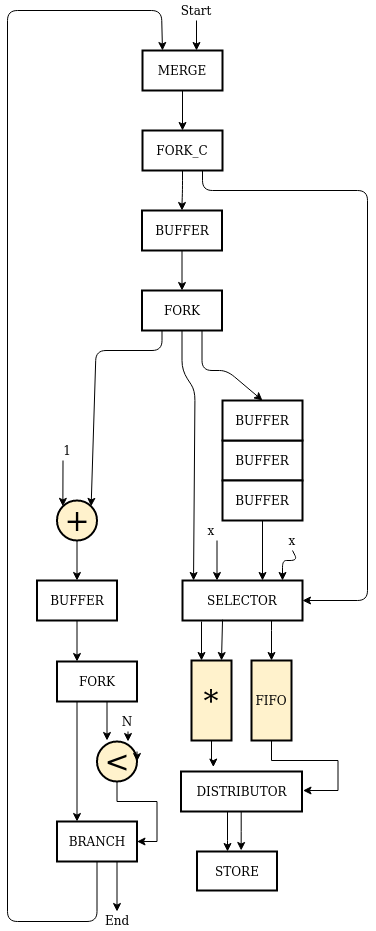
\includegraphics[scale=0.25]{blocking_shared_solution.png}
    \end{column}
  \end{columns}
\end{frame}

\begin{frame}{Ordering}
\begin{columns}
    \begin{column}{0.45\textwidth}
    We must enforce that all transactions from one BB happen before any from another BB (or the same in another iteration) \newline \newline
    We use the same mechanism as LSQs to be informed of ...
    \end{column}
    \begin{column}{0.1\textwidth}
    \end{column}
    \begin{column}{0.45\textwidth}
      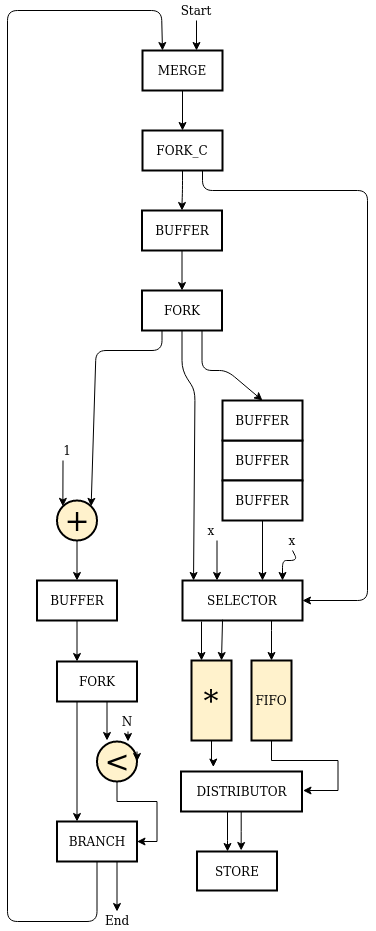
\includegraphics[scale=0.25]{blocking_shared_solution.png}
    \end{column}
  \end{columns}
\end{frame}

\begin{frame}{Selector}
Four new AST nodes :
\begin{itemize}
    \item MutVar
    \item Loop
    \item Branch
    \item Assign
\end{itemize}
\end{frame}

\begin{frame}{Distributor}
    Funsig that knows if tail rec or not
\end{frame}

\end{document}